\begin{figure}
  \centering
  \vskip -0.25cm
  \begin{tikzpicture}
    \node at (0, 0){
      \includegraphics[width=5cm]{experiments/2d/ppca_occ_dl/easy_5_bce/results}
    };
    \node at (0, -4){
      \includegraphics[width=5cm]{experiments/2d/vae_occ_dl/easy_5_bce/results_only}
    };
    \node at (-1.5, -6.5){
      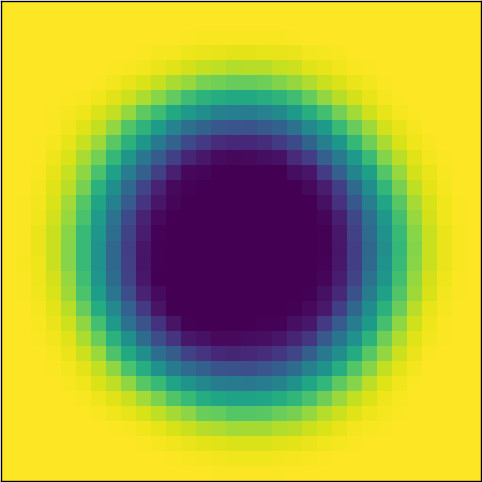
\includegraphics[height=2cm]{experiments/2d/vae_occ_dl/hard_5_bce_statistics/inference_statistics}
    };
    \node at (0, -9){
      \includegraphics[width=5cm]{experiments/2d/vae_evae/easy_5/results_only}
    };
    
    \draw[-,dashed] (2.75, -12.75) -- (2.75,3);
    
    \node at (5.5, 0){
      \includegraphics[width=5cm]{experiments/2d/ppca_occ_dl/hard_5_bce/results}
    };
    \node at (5.5, -4){
      \includegraphics[width=5cm]{experiments/2d/vae_occ_dl/hard_5_bce/results_only}
    };
    \node at (5.5, -6.5){
      \includegraphics[width=5cm]{experiments/2d/vae_occ_dl/hard_5_bce_statistics/results_only}
    };
    \node at (5.5, -9){
      \includegraphics[width=5cm]{experiments/2d/vae_evae/hard_5/results_only}
    };
    \node at (5.5, -11.5){
      \includegraphics[width=5cm]{experiments/2d/vae_evae/hard_5_statistics/results_only}
    };
    
    \node at (8.5,0) {
      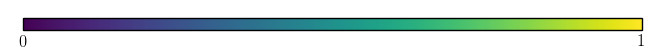
\includegraphics[height=5.5cm]{experiments/2d/vae_occ/colorbar}
    };
    
    \node[rotate=90] at (-3,-1.5) {\AML \PPCA};
    \node[rotate=90] at (-3,-4) {\AML \VAE};
    \draw[-,dashed] (-3,-2.75) -- (8.5,-2.75);
   
    \node[rotate=90] at (-3,-6.5) {\AML \VAE *};
    \draw[-,dashed] (-3,-5.25) -- (8.5,-5.25);
    
    \node[rotate=90] at (-3,-9) {\EVAE};
    \draw[-,dashed] (-3,-7.75) -- (8.5,-7.75);
   
    \node[rotate=90] at (-3,-11.5) {\EVAE *};
    \draw[-,dashed] (-3,-10.25) -- (8.5,-10.25);
    
    \node at (0, 3) {\easy};
    \node at (5.5, 3) {\hard};
  \end{tikzpicture}
  
  % TODO short caption
  \caption{Qualitative results for \AML and \EVAE. For \AML we additionally
  compare a \PPCA and a \VAE prior.
  The two  major columns show results for the \easy and \hard cases, respectively;
  each showing five samples. The top rows show the observed points, the
  corresponding free space and the targets. For each method, we show the
  corresponding predictions and their errors; see the text for details.}
  \label{fig:experiments-2d-aml-qual}
\end{figure}
